\Aufgabe{Zylinder}

  Ein (Kreis-)Zylinder ist definiert durch die H\"ohe $h$ und den
  Radius $r$ der Grundfl\"ache $G$.

  Ein Hohlzylinder (auch Rohr, engl. \emph{pipe}) ist definiert durch die
  H\"ohe $h$, den Au\ss enradius $R$ und den Innenradius $r$.

  \begin{figure}[h]
    \centering
    \subfigure[Zylinder]{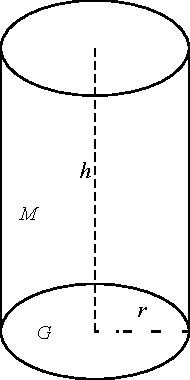
\includegraphics{../PUeUebungen/Scheme/Pue01/cylinder_fig}}
    \hfil
    \subfigure[Hohlzylinder]{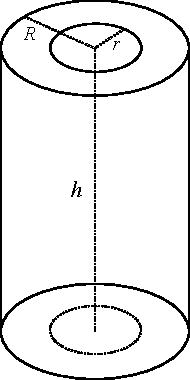
\includegraphics{../PUeUebungen/Scheme/Pue01/pipe_fig}}
  \end{figure}

Schreiben Sie Prozeduren, die die Oberfl\"ache von Zylindern und
Hohlzylindern berechnen. Dabei sind folgende Teilprobleme zu l\"osen:

 \begin{enumerate}
   \item Schreiben Sie Prozeduren
     \texttt{circle-area} und \texttt{circle-perimeter}, die Fl\"ache
     und Umfang eines Kreises mit gegebenem Radius $r$ berechnen.

     Die Fl\"ache ergibt sich als $A=\pi r^2$, der Umfang als $U =
     2\pi r$. Erkennen und abstrahieren Sie Teilprobleme!

   \item Schreiben Sie eine Prozedur
     \texttt{cylinder-side-area}, die aus dem Radius $r$ der
     Grundfl\"ache und der H\"ohe $h$ die Mantelfl\"ache $M$ eines
     Zylinders berechnet. Die Mantelfl\"ache bezeichnet die seitliche 
     Fl\"ache, die durch die Grundfl\"achen begrenzt wird.

     Schreiben Sie au\ss erdem eine Prozedur \texttt{cylinder-area},
     die die Oberfl\"ache eines Zylinders berechnet.

   \item Schreiben Sie eine Prozedur
     \texttt{pipe-area}, die die Oberfl\"ache eines Hohlzylinders 
     berechnet. Gegeben sind dabei die H\"ohe $h$ des Hohlzylinders, 
     der Au\ss enradius $R$ und der Innenradius $r$.

     Benutzen Sie dazu Prozeduren, die Sie bereits definiert haben!
 \end{enumerate}


  Abgabe:    Programm \texttt{pipe-area.rkt}
  

    \begin{solution}
\pagebreak
\lstinputlisting[caption=Zylinderproblem - Lösung]{../PUeUebungen/Scheme/Pue01/pipe-area.rkt}     
  \end{solution}

